\documentclass[12pt, a4paper]{article}
\usepackage{fullpage, amsmath, graphicx, hyperref, csquotes}
\usepackage{float}
\begin{document}



    \begin{titlepage}
        \begin{center}

            \vspace*{3cm}
            {\LARGE \textbf{\textsc{ECE 411: Computer Organization \& Design}}} \\
            \vspace{.5cm}
            {\large \textbf{\textsc{MP4: Efficient Pipelined RISC-V Processor}}} \\
            \vspace{2cm}

            {\large \textbf{Team ``CRC''}} \\
            \vspace{.5cm}
            Hao Ren (\href{mailto:haor2@illinois.edu}{haor2@illinois.edu}) \\
            Zhirong Chen (\href{mailto:zhirong4@illinois.edu}{zhirong4@illinois.edu}) \\
            Ziyuan Chen (\href{mailto:ziyuanc3@illinois.edu}{ziyuanc3@illinois.edu}) \\

            \vspace{1cm}
            \begin{table}[h]
                \centering
                \begin{tabular}{rl}
                    \hline
                    \textbf{Name} & \textbf{Contribution} \\
                    \hline
                    Hao Ren & Hazard Control Unit, Cacheline Prefetcher \\
                    Zhirong Chen & Processor Verification, Branch Predictor \\
                    Ziyuan Chen & Forwarding Unit, Arbiter, Customizable Cache \\
                    \hline
                \end{tabular}
            \end{table}

            \vspace{2cm}
            \textbf{Teaching Assistant:} Nicholas R. Satchanov \\
            \vspace{2cm}
            \textbf{Department of Electrical and Computer Engineering} \\
            \textbf{University of Illinois at Urbana-Champaign} \\
            \textbf{Champaign, Illinois 61820} \\
            \textbf{12/15/2023}

        \end{center}
    \end{titlepage}



    % -------------------------------------------------------------------------------- %



    \section{Introduction}
    This report encapsulates our exploratory journey in ECE 411, centered on the architectural development of a RISC-V based pipeline processor. Emphasizing the integration of advanced computer architecture features like enhanced branch prediction and multi-level cache systems, the project stands as a testament to our practical application of complex architectural concepts. This work not only aimed to build a high-performance processor but also served as a pivotal learning experience in understanding and applying computer architecture theories.

    Our report is organized into distinct sections for clarity and depth:
    \begin{enumerate}
        \item \textbf{Project Overview:} A broad perspective on the project’s goals and significance in modern computing.
        \item \textbf{Design Description:}
        \begin{itemize}
            \item \textbf{Overview:} General design philosophy and approach.
            \item \textbf{Milestones:}
            \begin{enumerate}
                \item \textbf{Checkpoint 1:} Initial design and implementation stages.
                \item \textbf{Checkpoint 2:} Intermediate developments and enhancements. Baseline pipeline processor finished.
                \item \textbf{Checkpoint 3:} Final stages and completion of the design with advanced features.
            \end{enumerate}
            \item \textbf{Advanced Design Options:} Detailed exploration of sophisticated features like branch prediction:
            \begin{itemize}
                \item \textbf{Design:} The architectural blueprint and rationale behind each feature.
                \item \textbf{Testing:} Methods and processes used to validate the design.
                \item \textbf{Performance Analysis:} Evaluation of the design's impact on processor performance based on energy and timing.
            \end{itemize}
        \end{itemize}
        \item \textbf{Conclusion:} Summary of our design objectives, achievements, and the novel aspects of our work.
    \end{enumerate}



    % -------------------------------------------------------------------------------- %



    \section{Project Overview}

    In our ECE 411 project, we designed and implemented a RV32I-based pipeline processor, focusing on incorporating advanced features to enhance its performance. The primary goal was to create a functional processor that also served as an educational tool through the integration of branch prediction, cache parameterization, and prefetching techniques.

    Branch prediction was crucial to mitigate performance degradation due to pipeline flushing. Cache parameterization and a multi-level cache system provided essential flexibility for performance optimization. The prefetcher, though ambitious, did not significantly improve performance as expected.
    
    The project demanded efficient team coordination, with responsibilities divided among members. Zhirong Chen and Ziyuan Chen took on the predictor and cache systems, while Hao Ren contributed to prefetcher, as well as integration and debugging. The project was challenging due to tight schedules and the need to balance advanced techniques with realistic goals. Ultimately, our collaborative effort led to a processor that surpassed our expectations, showcasing our design capabilities and learning.


    % -------------------------------------------------------------------------------- %



    \section{Milestones}

    \subsection{Checkpoint 1}
    \textbf{Purpose}: Implement the basic pipeline processor with 5 stages: IF, ID, EX, MEM, and WB. Finish the design of processor with datapath and control module. 
    
    Key features include maintaining each stage of the process for two cycles to accommodate memory requirements, integrated testing for CPU, and ensuring proper functionality of hazard controls. The data path involves pipeline registers and hardware logics, with cross-verification of comb logic and integrated tests as a processor. Control words are propagated from instruction to ensure complete information at each stage, including monitoring, with tests to verify appropriate propagation and integration.

    
    \begin{figure}[H]
        \centering
        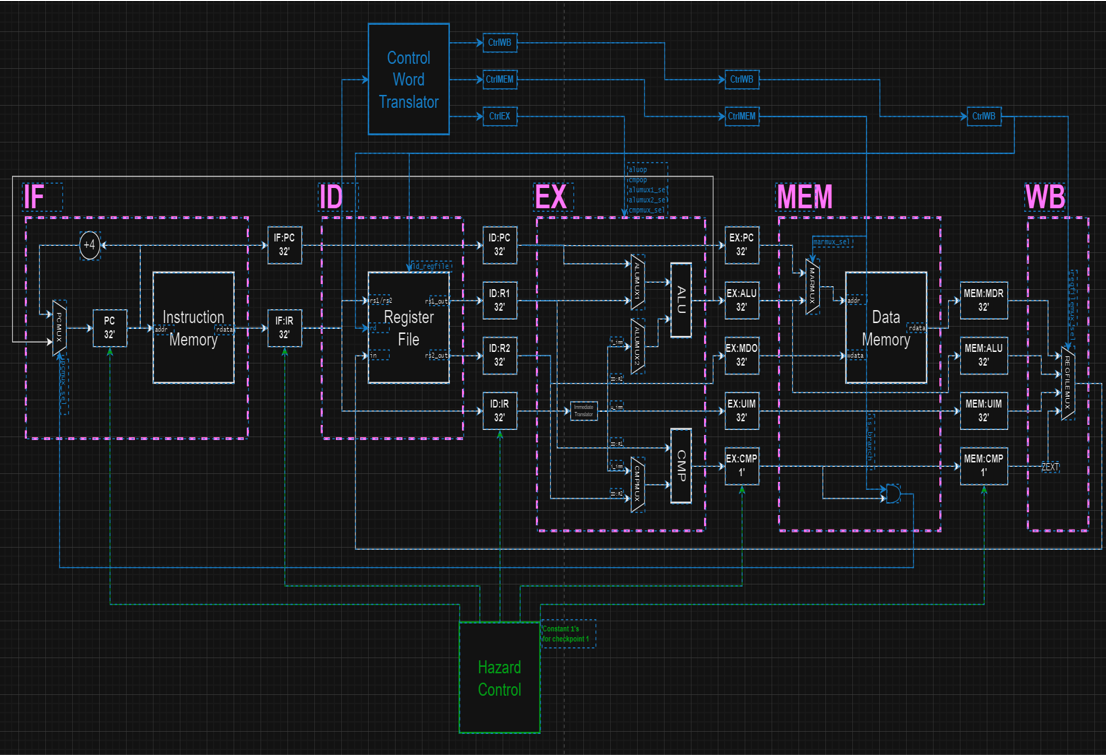
\includegraphics[width=0.8\textwidth]{pipeline_datapath.png}
        \caption{Pipeline Processor Datapath}
        \label{fig:enter-label}
    \end{figure}

    \begin{figure}[H]
        \centering
        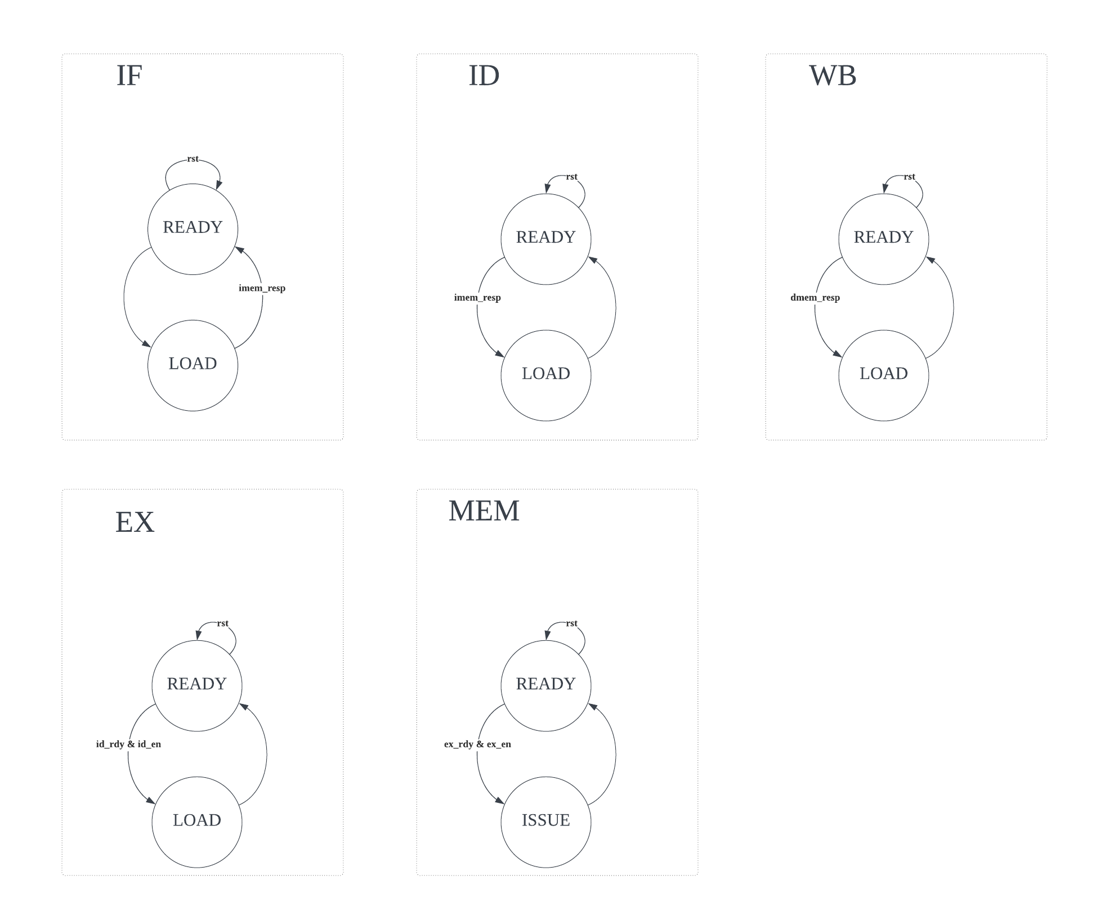
\includegraphics[width=0.8\textwidth]{state_transfer.png}
        \caption{Hazard Control State Transfer Diagram}
        \label{fig:enter-label}
    \end{figure}

    \textbf{Verification Strategy}: 

    \textit{Hazard Detection}:
    \begin{itemize}
        \item Functionality includes catching hazards and inserting bubbles.
        \item Inputs: Current instruction for IR register at IF ID and sets of (rs1 rs2 rd).
        \item Outputs: Decision to stall IF and insert bubble or allow pipeline flow, number of bubbles inserted.
        \item Verification: Testing different input combinations to assess hazard detection.
    \end{itemize}
    
    
    

    
    
\textit{Hazard Detection without Forwarding}:
\begin{itemize}
    \item Functionality focuses on forwarding data to eliminate bubbles.
    \item Same input and output considerations as Hazard Detection without forwarding.
    \item Verification involves reusing the previous DUT test.
\end{itemize}




    \subsection{Checkpoint 2}

    \textbf{Purpose}: Implement the arbiter, advanced hazard control, fast forwarding. 

    \textbf{Forwarding Unit}: The forwarding unit's main goal is to mitigate data hazards that occur when an instruction depends on the result of a previous instruction that has not yet completed its execution. In a pipelined processor, subsequent instructions can be in different stages of execution (like execution (EX), memory access (MEM), or write-back (WB)) simultaneously. These occur when instructions that are close together in a sequence modify and read the same data. 

    \textbf{Hazard Control Unit}: The unit detects and controls various types of hazards (like data hazards, control hazards) that can occur due to the concurrent execution of instructions in a pipeline. It manages the state of each pipeline stage (IF, ID, EX, MEM, WB) and determines whether they are ready (RDY) or busy (BUSY) based on the current instruction flow and hazard conditions. The unit generates commit signals for each pipeline stage, indicating whether the current stage can pass its result to the next stage in the pipeline. The unit includes logic to handle branch mispredictions, which is a form of control hazard. This involves resetting or disabling certain pipeline stages when a branch misprediction is detected. It controls the enabling of various pipeline stages based on the current state of the pipeline and the presence of hazards. This is essential for ensuring correct execution order and data integrity.

    \textbf{Arbiter}: The arbiter module you've provided is designed to manage access to a shared memory resource (referred to as pmem in the code) in a system where there are two potential requestors - instruction processing memory (ipmem) and data processing memory (dpmem). 

    \textbf{Testing Strategy}: For this design, we first use testbench for each module to test its functionality. For arbiter, we simulate the signal from cpu and memory to test its function. For forwarding unit, we design some scenarios of data dependency to test its functionality. Finally, we insert the forwarding unit to our design to test the whole functionality. We use branch.s arith.s and load\_store.s to test the pipeline processor functionality. 

    \textbf{Diagram}:

    \begin{figure}[H]
        \centering
        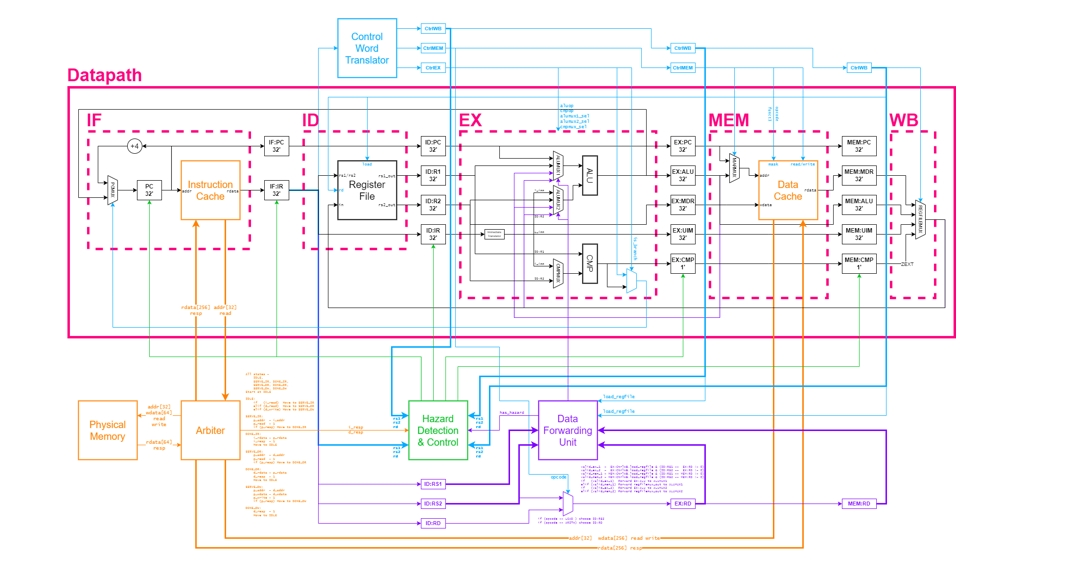
\includegraphics[width=0.76\textwidth]{forwarding_unit.png}
        \caption{Fowarding Unit}
        \label{fig:enter-label}
    \end{figure}

    
    \begin{figure}[H]
        \centering
        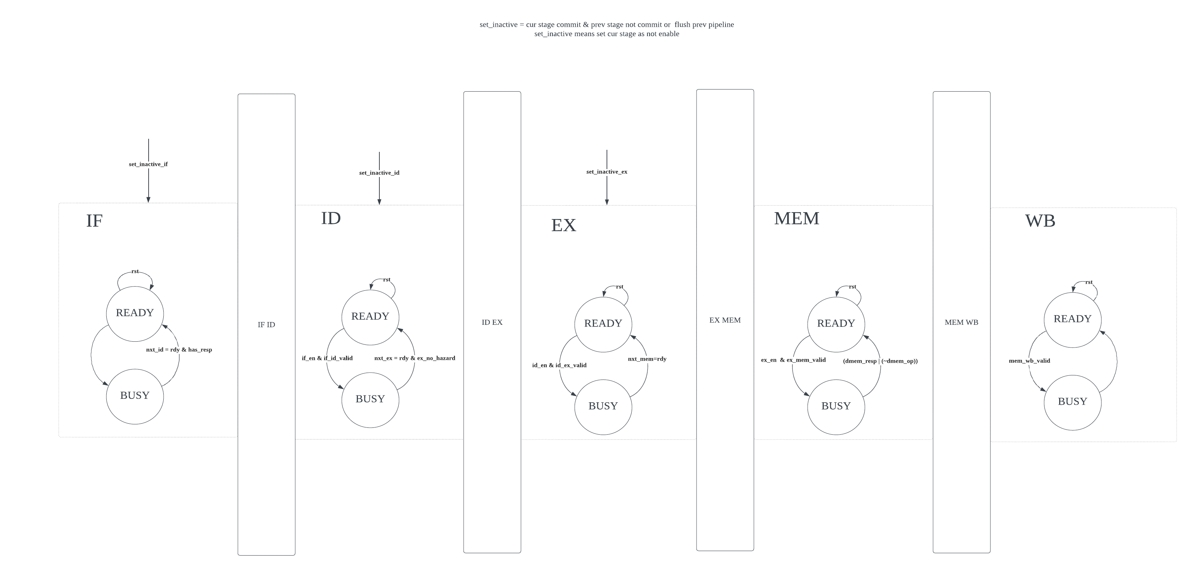
\includegraphics[width=0.75\textwidth]{hazard_control.png}
        \caption{Fowarding Unit}
        \label{fig:enter-label}
    \end{figure}


    \begin{figure}[H]
        \centering
        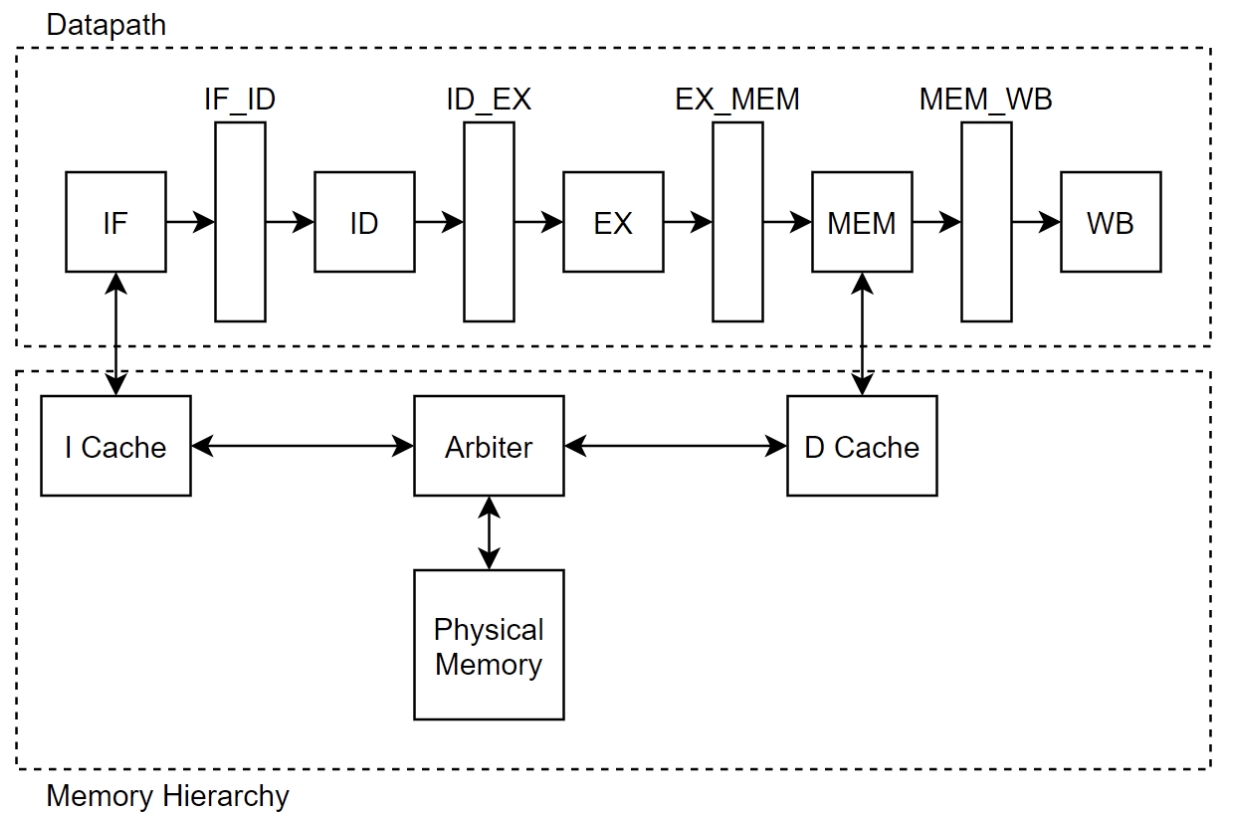
\includegraphics[width=0.75\textwidth]{arbiter.png}
        \caption{Fowarding Unit}
        \label{fig:enter-label}
    \end{figure}
    
    
    
    
    \subsection{Checkpoint 3}

    Checkpoint 3 marked a significant phase in the evolution of our RV32I-based pipeline processor, where we focused on enhancing key features and optimizing performance.

    \textbf{Design Overview:}
    Our efforts in this stage were directed towards refining the pipeline processor with local / global branch prediction, a multi-level cache, fully customizable cache, branch predictors, and prefetchers. The advancements made in these areas were critical in elevating the processor's efficiency and performance.
    
    \textbf{Advanced Feature Implementation:}
    \begin{itemize}
        \item \textbf{Branch Prediction:} We improved both local and global branch predictors, including a 4-way associated branch target buffer. The local predictor used the PC to index the Pattern History Table (PHT), while the global predictor employed a Branch History Register (BHR) for indexing.
        \item \textbf{Cache System:} The cache system was made highly customizable with parameters like word size, sets, and associativity, offering optimal configuration given the design constraints.
        \item \textbf{Prefetcher:} The next-line prefetcher was an ambitious addition, designed to improve performance by utilizing idle time in data and instruction memory. However, the prefetcher's impact was less significant than anticipated.
    \end{itemize}
    
    \textbf{Testing and Verification:}
    We conducted extensive testing to ensure the proper functioning of each component. This included:
    \begin{itemize}
        \item \textbf{Prefetcher Testing:} Verifying its ability to improve performance, integration with the arbiter, and correct behavior in various scenarios.
        \item \textbf{Branch Predictor Testing:} Using a detailed strategy to evaluate prediction accuracy and response under different branch scenarios.
        \item \textbf{Cache System Testing:} Ensuring the cache hit and miss logic, replacement policy, write policy, and cache coherency operated as expected.
    \end{itemize}
    
    \textbf{Statistics \& Observations:}
    The CP3 report provided detailed statistics and observations, highlighting the impact of different configurations on performance metrics like IPC and cache efficiency. These insights were instrumental in guiding our optimization strategies for Checkpoint 4.
    
    \textbf{Diagrams and Schematics:}

    \textbf{Branch Predictor}:
    
    Global Branch Predictor:

    \begin{figure}[H]
        \centering
        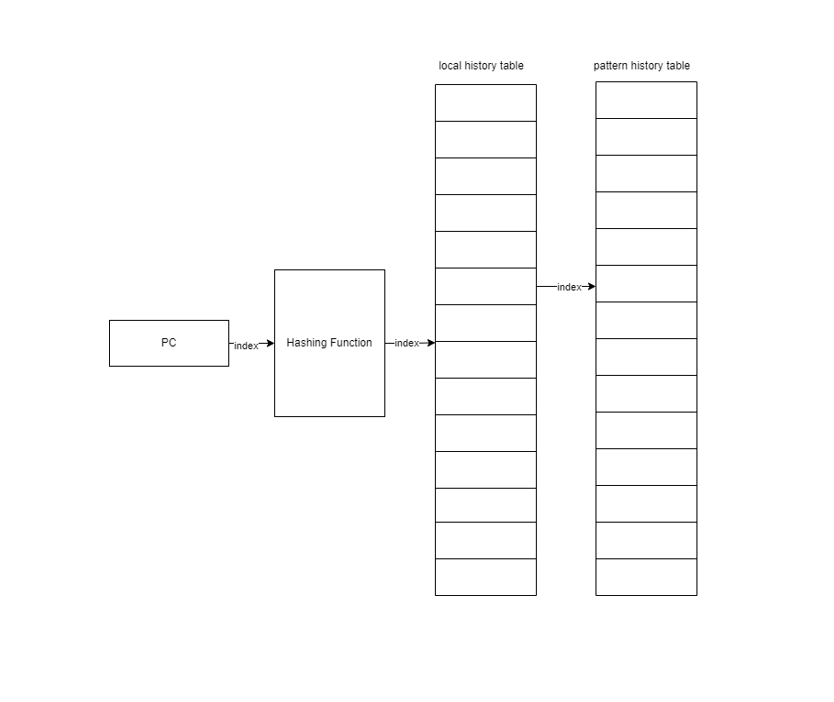
\includegraphics[width=0.75\textwidth]{local_branch_predictor.png}
        \caption{Local Branch Predictor}
        \label{fig:enter-label}
    \end{figure}

    \begin{figure}[H]
        \centering
        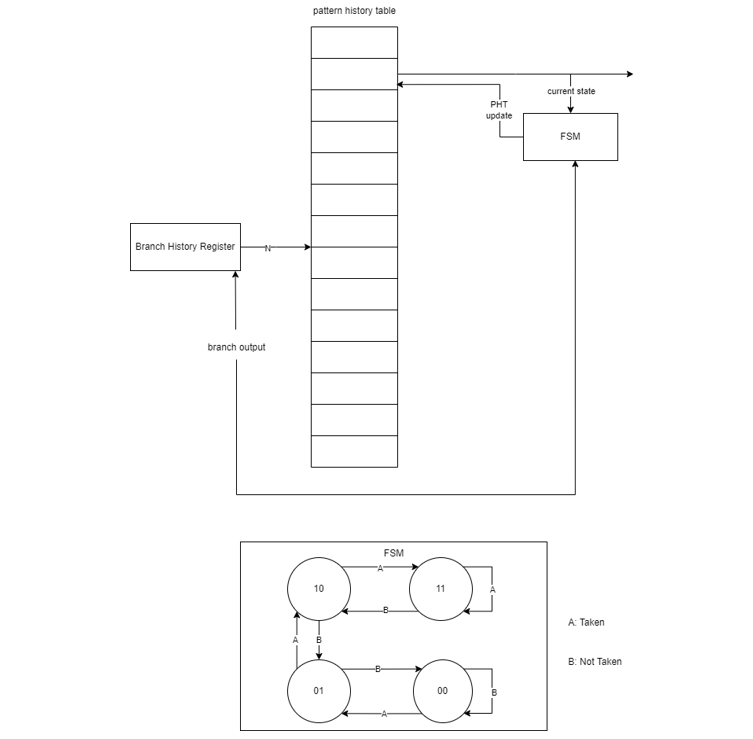
\includegraphics[width=0.65\textwidth]{global_branch_predictor.png}
        \caption{Global Branch Predictor}
        \label{fig:enter-label}
    \end{figure}

\textbf{Branch Target Buffer}:

    \begin{figure}[H]
        \centering
        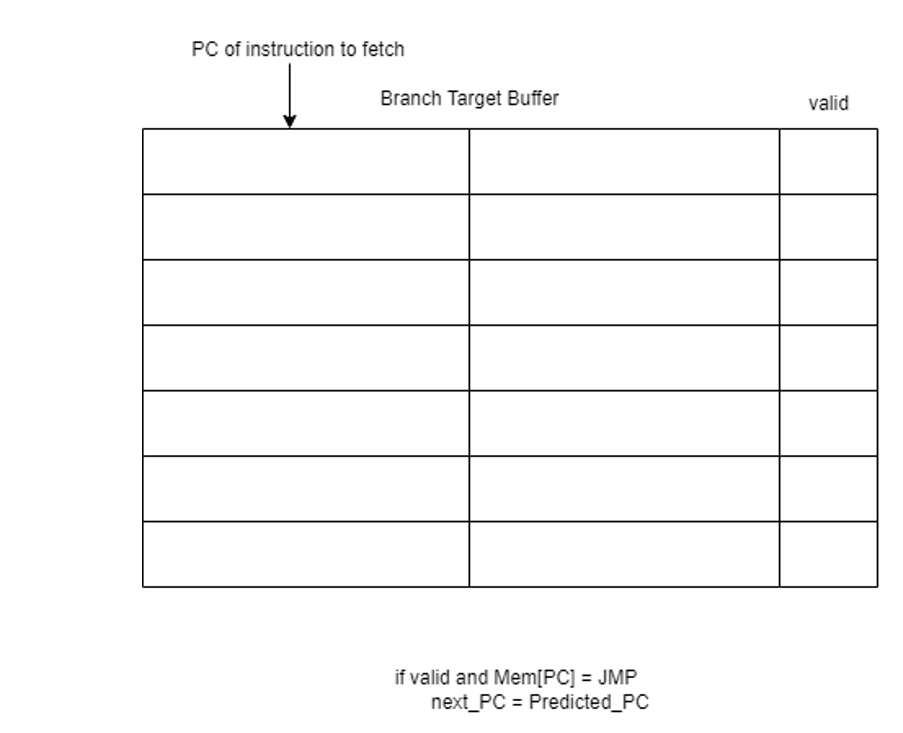
\includegraphics[width=0.75\textwidth]{branch_target_buffer.png}
        \caption{Branch Target Buffer}
        \label{fig:enter-label}
    \end{figure}

\textbf{Prefetcher}: 

    \begin{figure}[H]
        \centering
        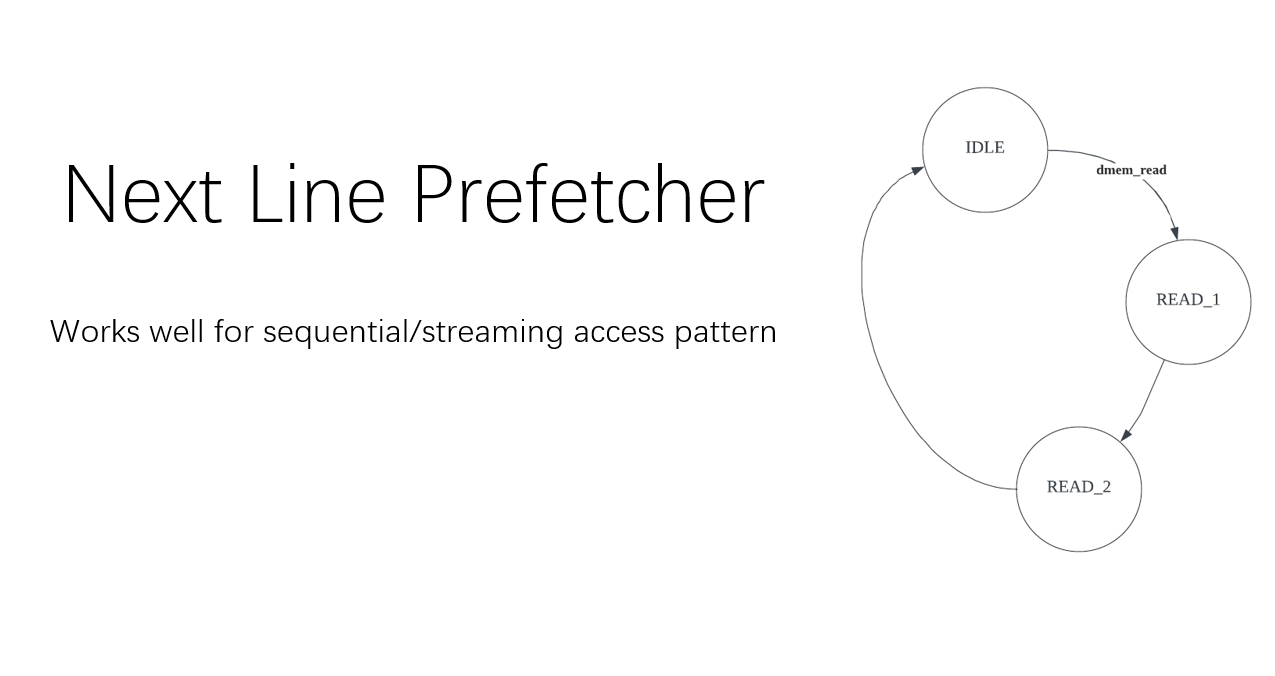
\includegraphics[width=0.75\textwidth]{prefetcher.png}
        \caption{Fowarding Unit}
        \label{fig:enter-label}
    \end{figure}

\textbf{Multi-Level Cache}:

    \begin{figure}[H]
        \centering
        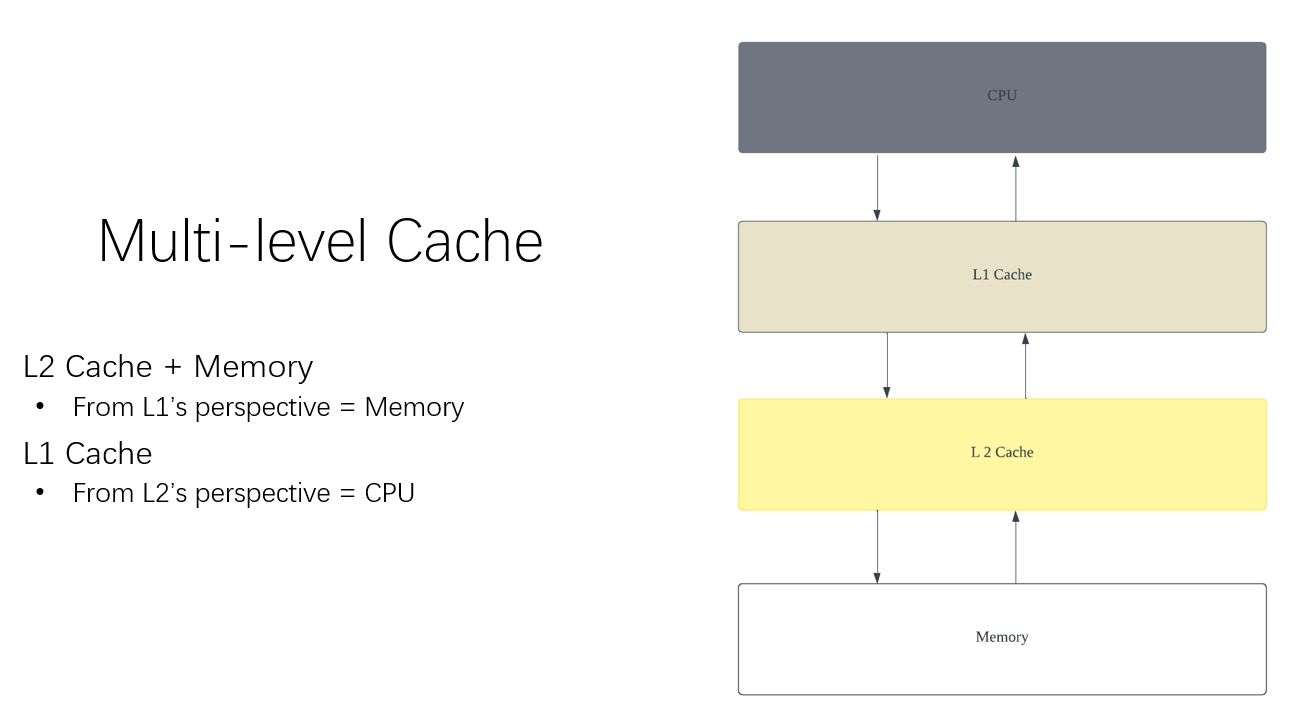
\includegraphics[width=0.75\textwidth]{multi_level_cache.png}
        \caption{Multi-Level Cache}
        \label{fig:enter-label}
    \end{figure}


    
    
    \textbf{Transition to Checkpoint 4:}
    As we move towards CP4, our focus will shift to further optimizing these features. This includes fine-tuning the cache parameters, refining the prefetching strategy, and exploring advanced predictors like the Tournament Predictor and G-Share Predictor.




    % -------------------------------------------------------------------------------- %



    \section{Advanced Design Features}

    \subsection{Branch Predictor}

    \textbf{Design and Implementation:}
    Zhirong Chen's work focused on implementing and refining both local and global branch predictors. The local branch predictor (LBP) utilized a Pattern History Table (PHT) indexed by the Program Counter (PC) to predict branch behavior, while the global branch predictor (GBP) used a Branch History Register (BHR) for indexing the PHT. A key aspect of our design was the integration of a 4-way associate Branch Target Buffer (BTB) to record and provide branch targets.
    
    \textbf{Performance Analysis:}
    Comparative performance data provided valuable insights:
    
    \begin{itemize}
        \item \textbf{Baseline (Static Predictor) with Prefetcher:}
        \begin{itemize}
            \item IPC: 0.236838, Branch Mispredict: 70.891\%
        \end{itemize}
        \item \textbf{Local Predictor with Prefetcher:}
        \begin{itemize}
            \item IPC: 0.275292, Branch Mispredict: 36.292\%
        \end{itemize}
        \item \textbf{Local Predictor with 4-Way BTB and Prefetcher:}
        \begin{itemize}
            \item IPC: 0.239635, Branch Mispredict: 67.810\%
        \end{itemize}
        \item \textbf{Local Predictor without Prefetcher:}
        \begin{itemize}
            \item IPC: 0.275790, Branch Mispredict: 36.277\%
        \end{itemize}
        \item \textbf{Global Predictor without Prefetcher:}
        \begin{itemize}
            \item IPC: 0.268125, Branch Mispredict: 42.378\%
        \end{itemize}
    \end{itemize}
    
    Our analysis indicated that both local and global predictors significantly reduced branch mispredictions compared to the static baseline. The global predictor, in particular, showed a balanced performance in terms of IPC and misprediction rate.
    
    \textbf{Trade-Offs:}
    The design involved trade-offs between complexity and performance. While the local predictor was simpler and faster, the global predictor offered better accuracy in varied branching scenarios. The integration of the BTB further complicated the design but provided faster target predictions for taken branches.
    
    \textbf{Impact on Workloads:}
    \begin{itemize}
        \item \textbf{Beneficial Workloads:} The branch predictors were especially effective in workloads with complex branching patterns, such as those found in control-intensive applications.
        \item \textbf{Challenges:} In workloads with unpredictable branching, the predictors' performance varied, with the global predictor generally performing better due to its broader historical perspective.
    \end{itemize}
    
    \textbf{Testing and Verification:}
    Comprehensive testing strategies were employed for both predictors:
    \begin{itemize}
        \item \textbf{LBP Testing:} Included initialization, branch taken and not taken tests, waveform analysis, and continuous monitoring.
        \item \textbf{GBP Testing:} Focused on evaluating prediction accuracy, learning ability, adaptation to changing patterns, and stress testing under rapidly changing branch directions.
    \end{itemize}
    
    \textbf{Conclusion:}
    The branch predictors significantly enhanced our processor's performance by reducing branch misprediction rates. The choice between local and global predictors depended on the specific workload characteristics, with the global predictor providing a more robust solution for diverse branching behaviors.


    \subsection{Cacheline Prefetcher}

    \textbf{Design and Implementation:}
    The cacheline prefetcher, designed and implemented by Hao Ren, aimed to enhance processor performance by prefetching the next cacheline during periods when both the Data Memory (DMEM) and Instruction Memory (IMEM) were idle. The key to its implementation was modifying the arbiter to allow for memory preemption and recording the last cacheline read from IMEM. The prefetcher was engineered to not expose the prefetched cacheline to the CPU, ensuring that only relevant data was processed.
    
    \textbf{Performance Impact:}
    Our analysis reveals a nuanced impact of the cacheline prefetcher on overall processor performance. While the theoretical advantage of prefetching lies in its potential to reduce cache misses, our observations indicated a slight decrease in Instructions Per Cycle (IPC) from 0.27579 to 0.275292 when the prefetcher was enabled. This unexpected outcome can be attributed to:
    \begin{itemize}
        \item \textbf{Increased Cache Hit Latency:} The prefetcher introduced additional latency in cache hits, which, in our processor's context with few cache misses, led to a performance degradation rather than an improvement.
        \item \textbf{Inefficient Prefetching in Certain Workloads:} The conservative nature of the prefetcher meant it was less effective in scenarios where cache misses were already minimal, leading to unnecessary prefetching without tangible benefits.
    \end{itemize}
    
    \textbf{Trade-Offs:}
    The prefetcher's design involved trade-offs between potential speed gains through reduced cache misses and the additional latency introduced by prefetch operations. While theoretically beneficial in workloads with frequent cache misses, in scenarios with fewer cache misses, the prefetcher's impact was negligible or even detrimental.
    
    \textbf{Testing and Verification:}
    The prefetcher underwent rigorous testing to ensure its functionality and integration with the system. Key aspects of testing included:
    \begin{enumerate}
        \item \textbf{Prefetch Functionality Tests:} Verifying correct prefetch operation when DMEM and IMEM were idle and checking the integration with the arbiter.
        \item \textbf{Branch Prediction Integration:} Testing the prefetcher's response to the branch taken signal and its ability to record and use the last read IMEM cache line for prefetch decisions.
        \item \textbf{State Machine and Control Logic Verification:} Ensuring correct state transitions, especially the introduction of the prefetch state, and verifying that prefetched data was not exposed to the CPU.
    \end{enumerate}
    
    \textbf{Conclusion:}
    The cacheline prefetcher's implementation demonstrated the intricate balance required in processor design between adding new features and maintaining overall efficiency. While the prefetcher theoretically promised performance improvements, its practical application in our processor highlighted the complexities of memory operations and their impact on system performance.


    \subsection{Multi-Level and Customizable Cache}

    
    \textbf{Design and Implementation:}
    Ziyuan Chen's focus on multi-level and customizable cache aimed to bridge the gap between CPU speed and memory access times. The multi-level cache, comprising L1 and L2 caches, was designed to optimize data access speeds. The L1 cache, located on the CPU chip, offered the fastest access but was limited in size. The L2 cache, larger and slightly slower, served as an intermediate storage. The customizable cache allowed dynamic adjustment of parameters like size, block size, associativity, making it adaptable to a range of applications.
    
    \textbf{Performance Analysis:}
    Our experiments with different cache configurations yielded insightful results:
    
    \begin{itemize}
        \item \textbf{Baseline (L1 Cache Only, 256 Wordsize, 16 Sets, 4 Ways):} 
        \begin{itemize}
            \item IPC: 0.229373
            \item L1 I Cache: 1173571 hits, 1280 misses, 2361298 cycles (11.059 penalty)
        \end{itemize}
        \item \textbf{128 Wordsize, 64 Sets, 16 Ways:} 
        \begin{itemize}
            \item IPC dropped to 0.227675
            \item Increased L1 cache miss rate, resulting in performance degradation compared to the baseline.
        \end{itemize}
        \item \textbf{256 Wordsize, 128 Sets, 4 Ways:} 
        \begin{itemize}
            \item IPC: 0.229732
            \item Reduced L1 I cache miss dramatically, proving to be the optimal configuration within our constraints.
        \end{itemize}
        \item \textbf{Larger Word Sizes (512 and 1024):} 
        \begin{itemize}
            \item Increased miss penalties outweighed the benefits of reduced misses, leading to a drop in IPC.
        \end{itemize}
    \end{itemize}
    
    \textbf{Trade-Offs:}
    The design of the multi-level and customizable cache involved balancing the cache size, word size, and associativity against the cache miss penalty. The optimal configuration needed to minimize cache misses while keeping the penalty reasonable. Larger word sizes, while reducing the number of misses, introduced heavier penalties which, in turn, adversely affected the IPC.
    
    \textbf{Impact on Workloads:}
    \begin{itemize}
        \item \textbf{Beneficial Workloads:} Workloads with frequent access to a variety of data benefit from the larger word sizes and sets, as they reduce cache misses.
        \item \textbf{Less Effective Workloads:} Workloads with smaller, more frequent data accesses may not benefit as much from larger caches due to the higher miss penalty.
    \end{itemize}
    
    \textbf{Testing and Verification:}
    Comprehensive testing strategies were implemented, including cache hit and miss tests, replacement policy tests, write policy tests, and cache coherency tests. These ensured the cache system operated as expected under various scenarios.
    
    \textbf{Conclusion:}
    The multi-level and customizable cache demonstrated significant improvements in data access times and system performance. The flexibility in cache configuration allowed for optimizations tailored to specific workloads, showcasing the effectiveness of a well-designed cache system in modern processors.




    % -------------------------------------------------------------------------------- %



    \section{Conclusion}

    Our journey in ECE 411 culminated in the successful design and implementation of a sophisticated RV32I-based pipeline processor. This project not only achieved its goal of creating a functional processor but also went beyond by integrating advanced features such as enhanced branch prediction, a multi-level cache system, and a cacheline prefetcher.

    Notable achievements include the significant reduction in branch misprediction rates through the implementation of both local and global branch predictors. The customizable cache system demonstrated our ability to optimize data access times, aligning with modern processor design practices. Although the prefetcher did not yield the expected performance boost, it offered valuable insights into the complexities of memory operations.
    
    A key aspect of our work was the balance between theoretical concepts and practical application, highlighted by the innovative design of the branch predictors and cache systems. These features not only enhanced our processor's efficiency but also served as a testament to our team's collaborative effort and problem-solving capabilities.
    
    In conclusion, this project stands as a testament to the effective application of computer architecture theories in a practical setting. Our processor, with its advanced features, not only meets the current standards of processor design but also opens avenues for future innovations in the field.



\end{document}
